%% Charlie Redmon
%% 20170907
%% SEM path diagram: [fill in description]

% standalone class for individual image to be included in a document
% border=15pt controls the whitespace padding around the diagram
\documentclass[border=15pt]{standalone}

% load custom style configurations from separate file
%% ------------------------------------------------------------
%% Charlie Redmon
%% 20170923
%% semTikzStyle.tex: style configurations for SEM path diagrams
%% ------------------------------------------------------------

\usepackage{tikz}

% observed variable
\tikzstyle{ov}=[shape=rectangle,
                draw=black!80,
                minimum height=0.6cm,
                minimum width=0.6cm,
                thick]

% response variable
\tikzstyle{av}=[shape=rectangle,
                draw=black!80,
                fill=black!10,
                minimum height=0.6cm,
                minimum width=0.6cm,
                thick]

% latent variable
\tikzstyle{lv}=[shape=circle,
                draw=black!80,
                thick,
                minimum width=1cm]

% correlations
\tikzstyle{lcor}=[bend left=30, dashed]
\tikzstyle{rcor}=[bend right=30, dashed]

% self-loops (for variance)
\tikzstyle{lloop}=[loop left, 
                   out=210, 
                   in=150, 
                   distance=0.3cm,
                   densely dotted]

\tikzstyle{rloop}=[loop right, 
                   out=30, 
                   in=-30, 
                   distance=0.3cm,
                   densely dotted]

\tikzstyle{aloop}=[loop above, 
                   out=60, 
                   in=120, 
                   distance=0.3cm,
                   densely dotted]

\tikzstyle{bloop}=[loop below, 
                   out=-60, 
                   in=-120, 
                   distance=0.3cm,
                   densely dotted]




\begin{document}

%% ">=stealth" sets the arrow head style
%% "semithick" sets the line width (0.6 pt)
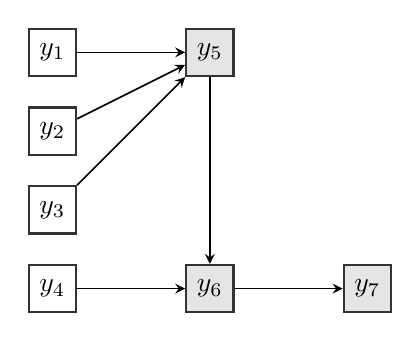
\begin{tikzpicture}[>=stealth,semithick]

\node[ov] (x1)                {$y_1$};
\node[ov] (x2) [below of=x1]  {$y_2$};
\node[ov] (x3) [below of=x2]  {$y_3$};
\node[ov] (x4) [below of=x3]  {$y_4$};

\begin{scope}[xshift=2cm]
\node[av] (x5) at (0,0)    {$y_5$};
\node[av] (x6) at (0,-3)   {$y_6$};
\end{scope}

\begin{scope}[xshift=4cm]
\node[av] (x7) at (0,-3)  {$y_7$};
\end{scope}

\path[->] (x1) edge node[above,scale=0.6] {} (x5)
          (x2) edge node[above,scale=0.6] {} (x5)
          (x3) edge node[above,scale=0.6] {} (x5)
          (x4) edge node[above,scale=0.6] {} (x6)

          (x5) edge node[above,scale=0.6] {} (x6)

          (x6) edge node[above,scale=0.6] {} (x7);
\end{tikzpicture}


\end{document}